% ------------------------------------------------------------------------------------
\vspace{5mm}
{\color{lightgray} \hrule}
\begin{enumerate}
	\item Aplique el algoritmo de Metropolis-Hastings considerando como función objetivo la distribución normal bivariada:
	\begin{equation} \label{eq:1}
		f_{X_1,X_2} (\bar{x}) = \frac{1}{2\pi} \left| \Sigma \right|^{-\frac{1}{2}} \exp\left\{ -\frac{1}{2} (\bar{x} - \mu)^{'} \Sigma^{-1} (\bar{x} - \mu) \right\}
	\end{equation}
	donde
	\begin{equation} \label{eq:2}
		\mu = \binom{\mu_1}{\mu_2}, \quad \Sigma = 
		\begin{pmatrix}
			\sigma_{1}^2 & \rho\sigma_{1}\sigma_{2} \\
			\rho\sigma_{1}\sigma_{2} & \sigma_{2}^2
		\end{pmatrix}.
	\end{equation}
	Así, se tienen las siguientes distribuciones condicionales:
	\begin{equation} \label{eq:3}
		X_1 | X_2 = x_2 \sim \mathcal{N}\left( \mu_1 + \rho \frac{\sigma_{1}}{\sigma_{2}} (x_2 - \mu_2), \sigma_{1}^2 (1-\rho^2) \right),
	\end{equation}
	\begin{equation} \label{eq:4}
		X_2 | X_1 = x_1 \sim \mathcal{N}\left( \mu_2 + \rho \frac{\sigma_{2}}{\sigma_{1}} (x_1 - \mu_1), \sigma_{2}^2 (1-\rho^2) \right).
	\end{equation}
	Considere las siguientes propuestas:
	\begin{equation} \label{eq:5}
		q_{1} \left( (x_1^{'}, x_2^{'}) | (x_1, x_2) \right) = f_{X_1 | X_2} ( x_1^{'} | x_2 ) \cdot \mathbbm{1} (x_2^{'} = x_2),
	\end{equation}
	\begin{equation} \label{eq:6}
		q_{2} \left( (x_1^{'}, x_2^{'}) | (x_1, x_2) \right) = f_{X_2 | X_1} ( x_2^{'} | x_1 ) \cdot \mathbbm{1} (x_1^{'} = x_1).
	\end{equation}
	A partir del algoritmo MH usando Kerneles híbridos simule valores de la distribución normal bivariada, fijando $\sigma_{1} = \sigma_{2} = 1$, considere los casos $\rho = 0.85$ y $\rho =0.99$.
\end{enumerate}

\textcolor{BrickRed}{\it Respuesta:}

En el archivo \textcolor{mediumblue}{ejercicio1\_tarea8.py}, se comienza implementando la función \textit{contornos()}, la cual recibe una cadena de Markov simulada y grafica su trayectoria. Además, recibe los parámetros de una distribución normal bivariada y genera su gráfica de contornos. Es útil para comparar la concentración de la cadena en la región de interés.

A continuación, se implementa la función \textit{METROPOLIS\_HASTINGS\_HYBRID\_KERNELS()}, la cual aplica el algoritmo Metropolis-Hastings con kérneles híbridos para $K$ propuestas simulando una cadena de Markov en $\mathbb{R}^n$ y toma los siguientes argumentos:
\begin{itemize}
	\item La función objetivo $f$ (en este caso es la normal bivariada \eqref{eq:1}).
	\item Una lista de funciones que generan propuestas $[q_{1_{gen}}, \dots, q_{K_{gen}}]$, es decir, en este caso las expresadas en \eqref{eq:5} y \eqref{eq:6}.
	\item Lista de funciones que calculan la densidad de probabilidad de las propuestas $[q_{1_{pdf}}, \dots, q_{K_{pdf}}]$ (es decir, \eqref{eq:5} y \eqref{eq:6}). Es importante que se respete el mismo orden de la lista de funciones generadoras.
	\item Lista de probabilidades de seleccionar cada kernel de propuesta $[p_1,\dots,p_{K}]$. Es importante que se respete el mismo orden de la lista de funciones generadoras y que $\sum_{k} p_k =1$. Si no se da, se toman probabilidades iguales para cada kernel, i.e., $p_1=\cdots p_K = \frac{1}{K}$.
	\item El valor inicial $x_0$ en el soporte de la distribución objetivo.
	\item El número de iteraciones del algoritmo (casi siempre se usa $N = 10,000$).
\end{itemize}

La función regresa la cadena simulada en $\mathbb{R}^n$ e imprime la tasa de aceptación lograda y el conteo de aceptaciones por kernel. A continuación, se define la función \textit{objetivo()} la cual implementa la expresión \eqref{eq:1} y las propuestas:
\begin{itemize}
	\item \textit{prop1\_gen()}  y \textit{prop1\_pdf()}
	\item \textit{prop2\_gen()} y \textit{prop2\_pdf()}
\end{itemize}
las cuales implementan las propuestas \eqref{eq:5} y \eqref{eq:6}, así como su densidad de probabilidad respectiva. En estas funciones es importante notar que se respeta cuando se deja fija alguna de las variables ($x_{2}^{'}=x_2$ en la propuesta $1$ y $x_{1}^{'}=x_1$ en la propuesta $2$).

Finalmente, se ejecuta el código principal, en el cual se definen los parámetros para la normal bivariada objetivo: el problema pide tomar $\sigma_{1}=\sigma_{2}=1$ y para elegir $\mu_1$ y $\mu_2$, se eligieron de forma uniforme en $[0,10]$, resultando en $\mu_1=7.216$ y $\mu_2 = 0.077$ aunque se puede elegir donde sea necesario.

El punto $x_0$ inicial se tomó en $[10,2.5]$ y aunque teóricamente puede tomarse donde sea debido a que el soporte de la normal bivariada es todo $\mathbb{R}^2$, si se aleja mucho del punto $[\mu_1,\mu_2]$, puede causar indeterminaciones. Para el algoritmo Metropolis-Hastings, se usaron $100,000$ muestras y a ambas propuestas se les dio probabilidad de elección igual a $\frac{1}{2}$.

\begin{figure}[h] \label{fig:1}
	\centering
	\begin{minipage}{0.495\textwidth}
		\centering
		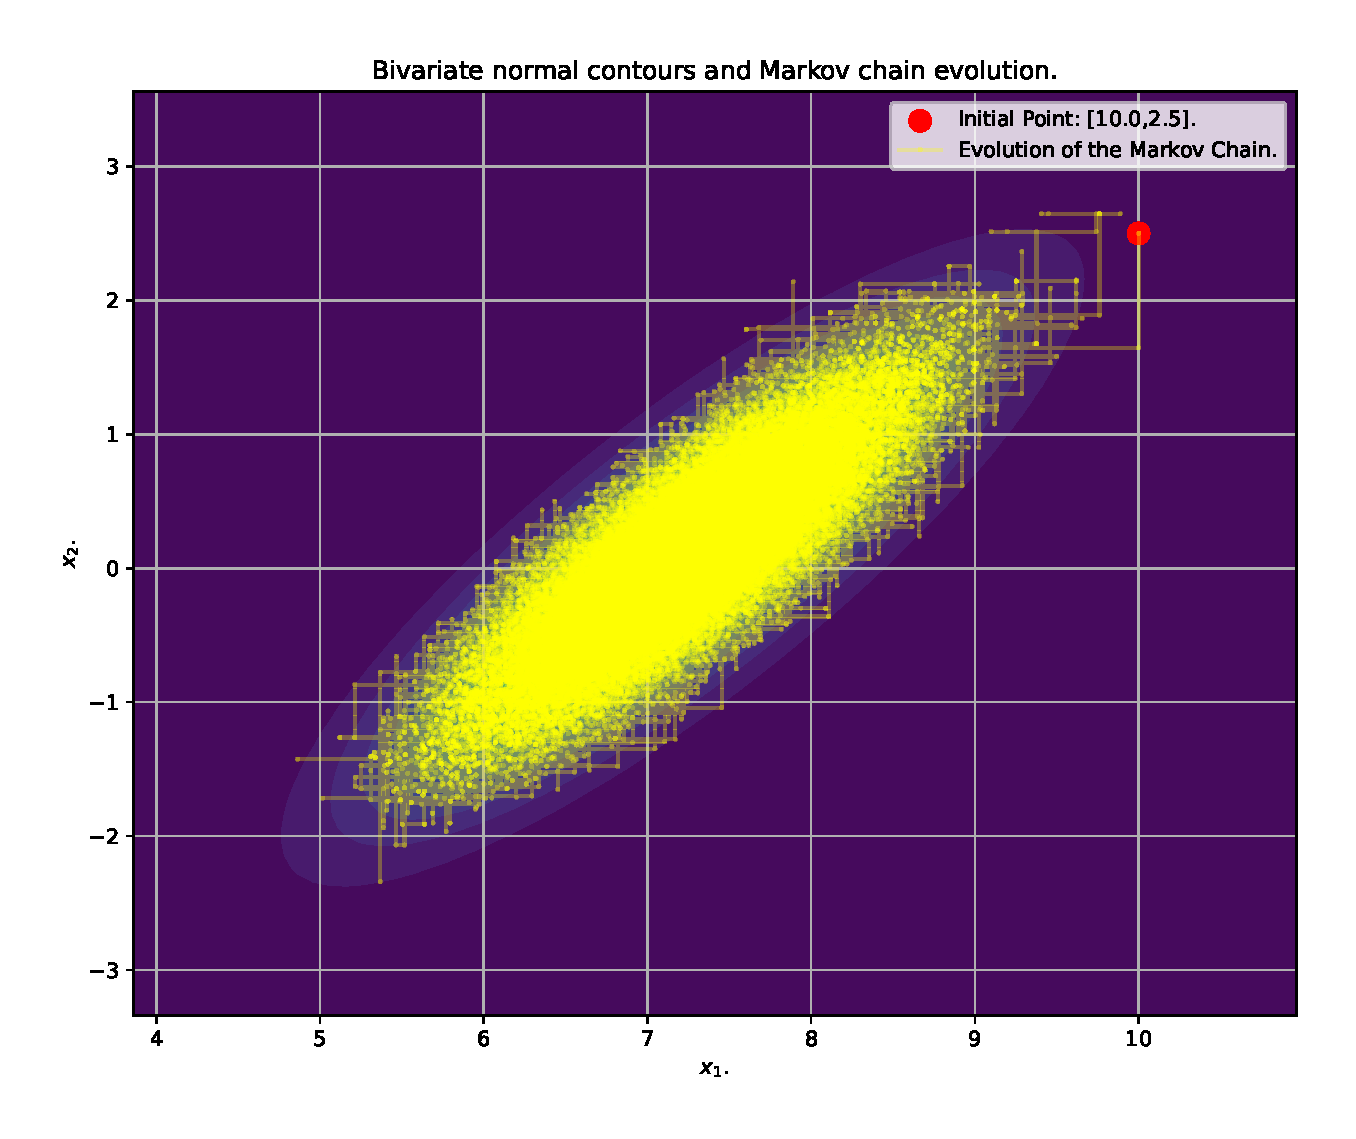
\includegraphics[width=\textwidth]{IMAGENES/p085.pdf}
		\caption{$\rho = 0.85$.}
	\end{minipage}
	\hfill
	\begin{minipage}{0.495\textwidth}
		\centering
		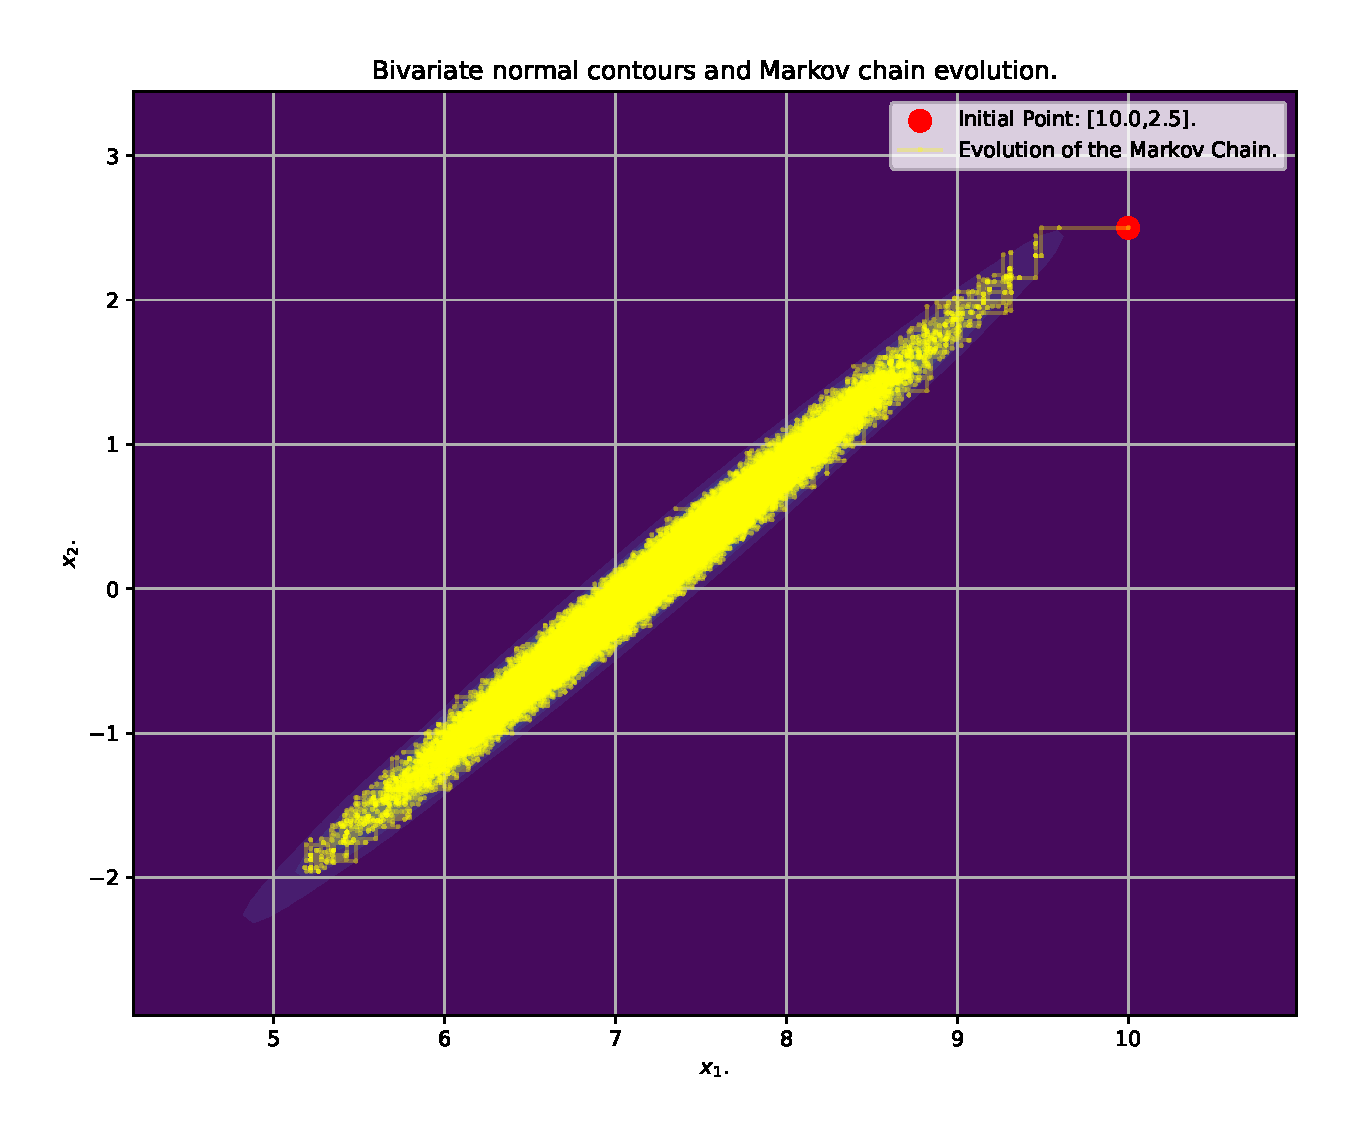
\includegraphics[width=\textwidth]{IMAGENES/p099.pdf}
		\caption{$\rho = 0.99$.}
	\end{minipage}
\end{figure}

Finalmente, para cada valor de $\rho \in \{0.85, 0.99\}$, se generaron las listas de funciones generadoras y sus respectivas densidades para aplicar el algoritmo Metropolis Hastings con Kérneles Híbridos generando los resultados mostrados en la figura anterior.

Sabemos que en una distribución normal bivariada, el coeficiente de correlación $\rho$ controla la dependencia lineal entre las dos variables aleatorias, afectando la forma de los contornos de la distribución conjunta. Es por esto que podemos notar que a medida que $\rho$ se acerca a 1, la dispersión en la dirección perpendicular a la correlación disminuye y la distribución se concentra más a lo largo de una línea, lo que explica el efecto de “concentración” que se observa en los datos simulados para $\rho = 0.99$ en comparación con $\rho = 0.85$.